\documentclass[border={0.1cm 0.1cm 0.1cm 0.1cm}]{standalone}  %E,S,W,N

\usepackage{amssymb}
\usepackage{amsmath}
\usepackage{tikz}
\usetikzlibrary{decorations.text}
\renewcommand{\familydefault}{\sfdefault}	%sans serif as default font

\begin{document}
	
	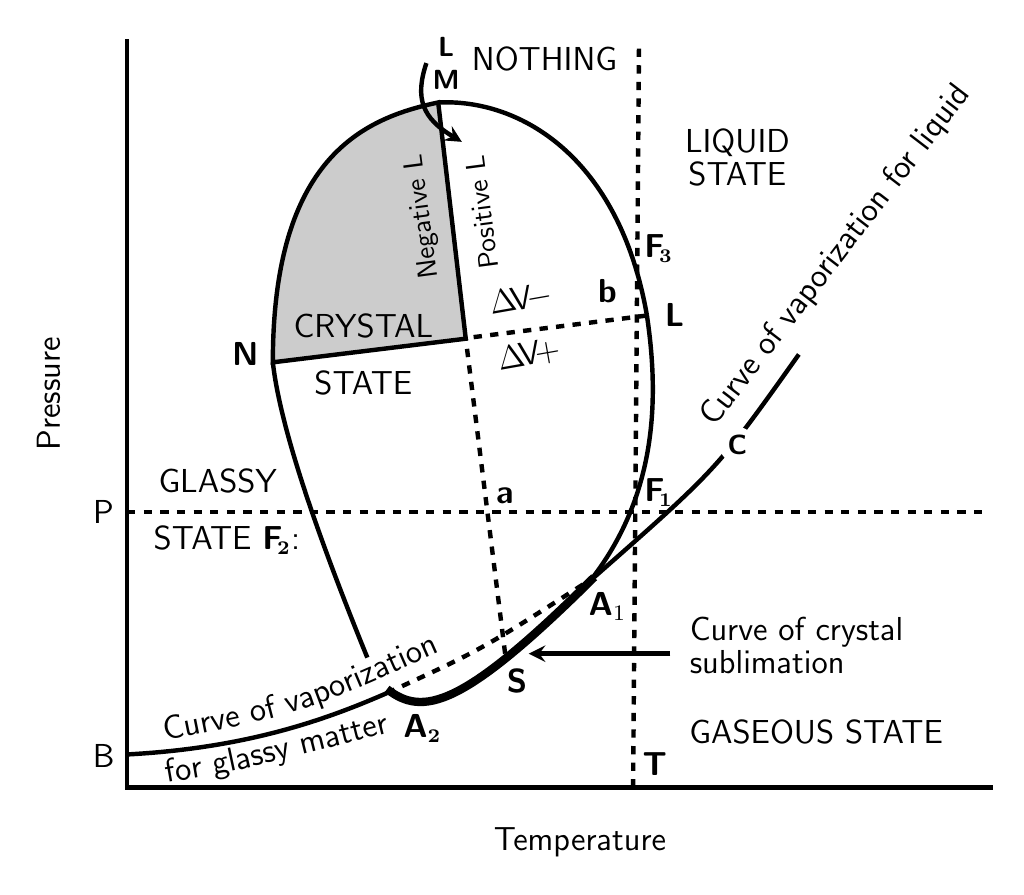
\begin{tikzpicture}[ultra thick]
	%AXIS
	\draw (0,9.5)--(0,0)--(11,0);
	\node at (5.75,-0.7) {\large Temperature};
	\node at (-1,5) {\rotatebox{90}{\large Pressure}};
	\draw[dashed] (0,3.5)--(10.9,3.5); %horizontal dash
	\draw[dashed] (6.425,0)--(6.5,9.4); %vertical dash
	\node at (-0.3,3.5) {\large P};
	\node at (-0.3,0.4) {\large B};
	
	%MAIN SHAPE
	\fill[opacity=0.2] (1.85,5.4) .. controls (1.85,8) and (3,8.5) .. (3.95,8.7) -- (4.3,5.7)--cycle;
	\draw (1.85,5.4) .. controls (1.85,8) and (3,8.5) .. (3.95,8.7)--(4.3,5.7)--cycle;
	%\draw (1.85,5.4)--(4.3,5.7)--(3.95,8.7); %_|
	\draw (3.95,8.7) .. controls (5,8.75) and (6.25,8) .. (6.6,6);
	\draw (6.6,6) .. controls (6.75,5) and (6.75,3.75) .. (5.9,2.65);
	\draw[line width=3] (5.93,2.67) .. controls (4.25,1) and (3.75,0.9) .. (3.3,1.25);
	\draw (3.05,1.65) .. controls (2.5,3) and (1.95,4.5) .. (1.85,5.4);
	%
	\draw (0,0.42) .. controls (1.5,0.5) and (2.5,0.85) .. (3.3,1.2); %B
	\draw[dashed] (3.3,1.2) .. controls (4.5,1.75) .. (5.9,2.65); %B dashed
	\draw (5.93,2.67) .. controls (7.5,4.05) .. (8.53,5.5);
	%
	\draw[dashed] (4.4,5.72)--(6.65,6);
	\draw[dashed] (4.8,1.7)--(4.3,5.7);
	
	%INNER LABELS
	\node[align=center] at (1.15,3.5) {\large GLASSY \\[3mm] \large $\;\;$STATE \textbf{F$\!_\textrm{\scriptsize 2}$}:};
	\node[align=center] at (3,5.5) {\large CRYSTAL \\[3mm] \large STATE};
	\node[align=center] at (7.75,8) {\large LIQUID \\ \large STATE};
	\node at (8.75,0.7) {\large GASEOUS STATE};
	\node at (5.3,9.25) {\large NOTHING};
	%
	\node[align=left,right] at (7,1.8) {\large Curve of crystal \\ \large sublimation};
		\draw[->,>=stealth] (6.9,1.7)--(5.1,1.7);
	\node at (6.1,2.3) {\large\bfseries A$_1$};
	\node at (3.75,0.75) {\large\bfseries A$_\textrm{\scriptsize 2}$};
	\node at (6.75,3.75) {\large\bfseries F$\!_\textrm{\scriptsize 1}$};
	\node at (6.75,6.85) {\large\bfseries F$\!_\textrm{\scriptsize 3}$};
	\node[align=center] at (4.05,9.2) {\bfseries L \\ \bfseries M};
		\draw[->,>=stealth] (3.8,9.2) .. controls (3.65,8.75) and (3.75,8.5) .. (4.25,8.2);
	\node at (6.95,6) {\large\bfseries L};
	\node at (4.95,1.35) {\large\bfseries S};
	\node at (4.8,3.7) {\large\bfseries a};
	\node at (6.1,6.3) {\large\bfseries b};
	\node at (1.5,5.5) {\large\bfseries N};
	\node at (6.7,0.3) {\large\bfseries T};
	\fill[white] (7.75,4.35) circle (6.5pt); \node at (7.75,4.35) {\bfseries C};
	\node at (9,6.75) {\rotatebox{52.5}{\large Curve of vaporization for liquid}};
	\node at (5,6.2) {\rotatebox{10}{\large $\Delta\!$V$\!-$}};
	\node at (5.1,5.5) {\rotatebox{10}{\large $\Delta\!$V$\!+$}};
	\node at (3.75,7.25) {\rotatebox{97.5}{Negative L}};
	\node at (4.5,7.3) {\rotatebox{97.5}{Positive L}};
	%
	\draw [decorate, decoration={text along path, text align=center, text={|\large|Curve of vaporization fo}}] (0.75,0.65) .. controls (2.25,0.95) .. (4.15,1.8);
	%\node at (1.5,0.35) {\rotatebox{10}{for glass}};
	\draw [decorate, decoration={text along path, text align=center, text={|\large|for glassy matter test}}] (1.25,0.19) .. controls (1.55,0.25) and (1.95,0.35) .. (3.35,0.7);
	%\draw[blue] (1.2,0.175) .. controls (1.5,0.25) and (1.9,0.3) .. (3.3,0.75);
	
	%\draw[help lines] (0,0) grid (11,9);
	\end{tikzpicture}
	
\end{document}